\documentclass[a4paper]{article}

% bloc : évite un changement de page
% completemulti : ajoute une case : aucune bonne réponse
%\newcommand{\repRel}{../..}
%\input{\repRel/Style/packages}
%%\input{\repRel/Style/new_style}
%\input{\repRel/Style/macros_SII}
%%\input{\repRel/Style/environment}

\usepackage[francais,bloc,completemulti,ensemble]{automultiplechoice}
%\usepackage[francais,bloc,completemulti]{automultiplechoice} 
\usepackage{amsmath}
% ensemble : feuille de questions et feuille de réponse séparées

\usepackage{multicol}

%% Pour le python %%
\usepackage{listingsutf8}

\lstset{language=Python,
  inputencoding=utf8/latin1,
  breaklines=true,
  basicstyle=\ttfamily\small,
  keywordstyle=\bfseries\color{green!40!black},
  commentstyle=\itshape\color{purple!40!black},
  identifierstyle=\color{blue},
  stringstyle=\color{orange},
  upquote = true,
  columns=fullflexible,
  backgroundcolor=\color{gray!10},frame=leftline,rulecolor=\color{gray}}  
  
\definecolor{mygreen}{rgb}{0,0.6,0}

\lstset{
     literate=%
         {é}{{\'e}}1    
         {è}{{\`e}}1    
         {ê}{{\^e}}1    
         {à}{{\`a}}1
         {â}{{\^a}}1		 
         {ô}{{\^o}}1    
         {ù}{{\`u}}1    
         {î}{{\^i}}1    
}
\lstset{inputpath=code}

\usepackage{siunitx}
%\usepackage[utf8x]{inputenc}
%\usepackage[T1]{fontenc}

\begin{document}
\AMCrandomseed{233893}
\setdefaultgroupmode{withoutreplacement} % Mélange des questions groupées

\graphicspath{{../../Banque_SI/03_hyperstatisme/images/}}
\element{mob}{
\begin{question}{mob 01}
Soit le schéma suivant. Donner la mobilité du mécanisme.
\begin{center}
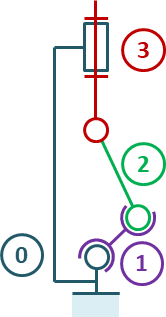
\includegraphics[width=3cm]{cas_01}
\end{center}
	\begin{reponses}	
	\bonne 2
	\mauvaise 0
	\mauvaise 1
	\mauvaise 3
	\end{reponses}
\end{question}\\}

\element{mob}{
\begin{question}{mob 02}
Soit le schéma suivant. Donner la mobilité du mécanisme.
\begin{center}
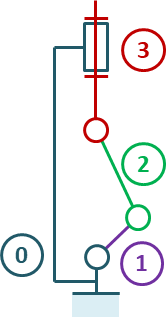
\includegraphics[width=3cm]{cas_02}
\end{center}
	\begin{reponses}	
	\bonne 0
	\mauvaise 1
	\mauvaise 2
	\mauvaise 3
	\end{reponses}
\end{question}\\}


\element{mob}{
\begin{question}{mob 03}
Soit le schéma suivant. Donner la mobilité du mécanisme.
\begin{center}
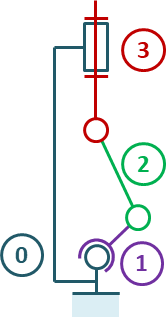
\includegraphics[width=3cm]{cas_03}
\end{center}
	\begin{reponses}	
	\bonne 1
	\mauvaise 0
	\mauvaise 2
	\mauvaise 3
	\end{reponses}
\end{question}\\}


\element{mob}{
\begin{question}{mob 04}
Soit le schéma suivant. Donner la mobilité du mécanisme.
\begin{center}
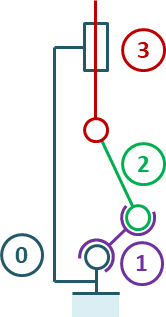
\includegraphics[width=3cm]{cas_04}
\end{center}
	\begin{reponses}	
	\bonne 3
	\mauvaise 0
	\mauvaise 1
	\mauvaise 2
	\end{reponses}
\end{question}\\}

\element{mob}{
\begin{question}{mob 05}
Soit le schéma suivant. Donner la mobilité du mécanisme.
\begin{center}
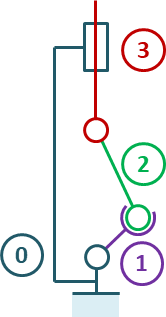
\includegraphics[width=3cm]{cas_05}
\end{center}
	\begin{reponses}	
	\bonne 1
	\mauvaise 0
	\mauvaise 2
	\mauvaise 3
	\end{reponses}
\end{question}\\}


\element{mob}{
\begin{question}{mob 06}
Soit le schéma suivant. Donner la mobilité du mécanisme.
\begin{center}
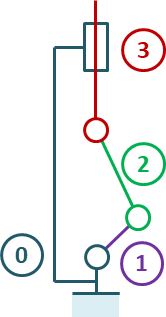
\includegraphics[width=3cm]{cas_06}
\end{center}
	\begin{reponses}	
	\bonne 1
	\mauvaise 0
	\mauvaise 2
	\mauvaise 3
	\end{reponses}
\end{question}\\}

\element{mob}{
\begin{question}{mob 07}
Soit le schéma suivant. Donner la mobilité du mécanisme.
\begin{center}
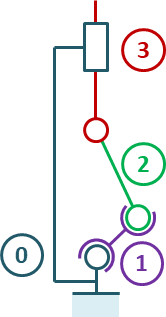
\includegraphics[width=3cm]{cas_07}
\end{center}
	\begin{reponses}	
	\bonne 2
	\mauvaise 0
	\mauvaise 1
	\mauvaise 3
	\end{reponses}
\end{question}\\}

\element{mob}{
\begin{question}{mob 08}
Soit le schéma suivant. Donner la mobilité du mécanisme.
\begin{center}
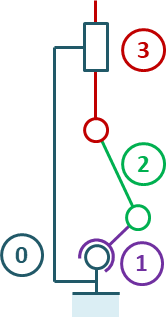
\includegraphics[width=3cm]{cas_08}
\end{center}
	\begin{reponses}	
	\bonne 1
	\mauvaise 0
	\mauvaise 2
	\mauvaise 3
	\end{reponses}
\end{question}\\}


\element{mob}{
\begin{question}{mob 09}
Soit le schéma suivant. Donner la mobilité du mécanisme.
\begin{center}
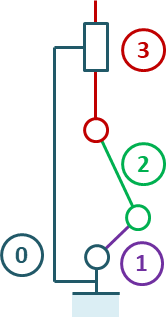
\includegraphics[width=3cm]{cas_09}
\end{center}
	\begin{reponses}	
	\bonne 3
	\mauvaise 0
	\mauvaise 1
	\mauvaise 2
	\end{reponses}
\end{question}\\}


\element{mob}{
\begin{question}{mob 10}
Soit le schéma suivant. Donner la mobilité du mécanisme.
\begin{center}
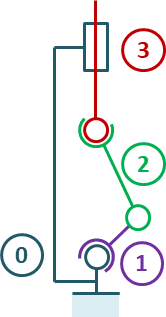
\includegraphics[width=3cm]{cas_10}
\end{center}
	\begin{reponses}	
	\bonne 3
	\mauvaise 0
	\mauvaise 1
	\mauvaise 2
	\end{reponses}
\end{question}\\}


\element{mob}{
\begin{question}{mob 11}
Soit le schéma suivant. Donner la mobilité du mécanisme.
\begin{center}
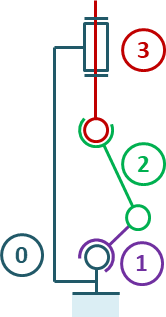
\includegraphics[width=3cm]{cas_11}
\end{center}
	\begin{reponses}	
	\bonne 2
	\mauvaise 0
	\mauvaise 1
	\mauvaise 3
	\end{reponses}
\end{question}\\}

\element{mob}{
\begin{question}{mob 12}
Soit le schéma suivant. Donner la mobilité du mécanisme.
\begin{center}
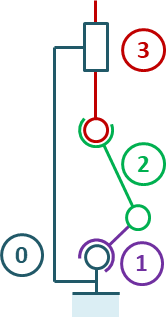
\includegraphics[width=3cm]{cas_12}
\end{center}
	\begin{reponses}	
	\bonne 2
	\mauvaise 0
	\mauvaise 1
	\mauvaise 3
	\end{reponses}
\end{question}\\}


\element{hs}{
\begin{question}{hs 01}
Soit le schéma suivant. Donner le degré d'hyperstatisme du mécanisme.
\begin{center}
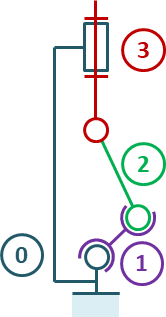
\includegraphics[width=3cm]{cas_01}
\end{center}
	\begin{reponses}	
	\bonne 0
	\mauvaise 1
	\mauvaise 2
	\mauvaise 3
	\end{reponses}
\end{question}\\}

\element{hs}{
\begin{question}{hs 02}
Soit le schéma suivant. Donner le degré d'hyperstatisme du mécanisme.
\begin{center}
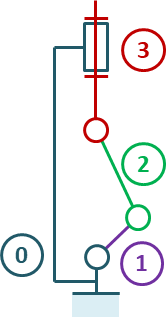
\includegraphics[width=3cm]{cas_02}
\end{center}
	\begin{reponses}	
	\bonne 2
	\mauvaise 0
	\mauvaise 1
	\mauvaise 3
	\end{reponses}
\end{question}\\}


\element{hs}{
\begin{question}{hs 03}
Soit le schéma suivant. Donner le degré d'hyperstatisme du mécanisme.
\begin{center}
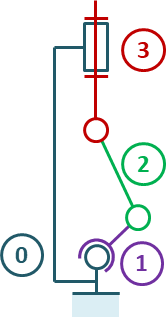
\includegraphics[width=3cm]{cas_03}
\end{center}
	\begin{reponses}	
	\bonne 1
	\mauvaise 0
	\mauvaise 2
	\mauvaise 3
	\end{reponses}
\end{question}\\}


\element{hs}{
\begin{question}{hs 04}
Soit le schéma suivant. Donner le degré d'hyperstatisme du mécanisme.
\begin{center}
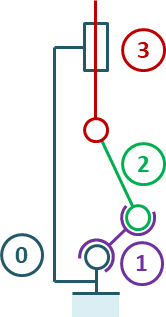
\includegraphics[width=3cm]{cas_04}
\end{center}
	\begin{reponses}	
	\bonne 0
	\mauvaise 3
	\mauvaise 1
	\mauvaise 2
	\end{reponses}
\end{question}\\}

\element{hs}{
\begin{question}{hs 05}
Soit le schéma suivant. Donner le degré d'hyperstatisme du mécanisme.
\begin{center}
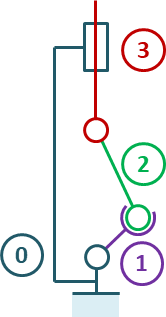
\includegraphics[width=3cm]{cas_05}
\end{center}
	\begin{reponses}	
	\bonne 0
	\mauvaise 1
	\mauvaise 2
	\mauvaise 3
	\end{reponses}
\end{question}\\}


\element{hs}{
\begin{question}{hs 06}
Soit le schéma suivant. Donner le degré d'hyperstatisme du mécanisme.
\begin{center}
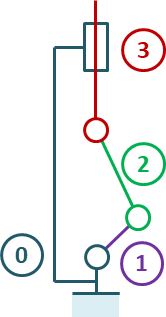
\includegraphics[width=3cm]{cas_06}
\end{center}
	\begin{reponses}	
	\bonne 2
	\mauvaise 0
	\mauvaise 1
	\mauvaise 3
	\end{reponses}
\end{question}\\}

\element{hs}{
\begin{question}{hs 07}
Soit le schéma suivant. Donner le degré d'hyperstatisme du mécanisme.
\begin{center}
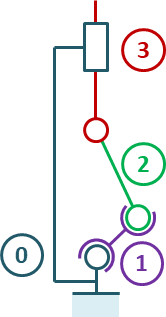
\includegraphics[width=3cm]{cas_07}
\end{center}
	\begin{reponses}	
	\bonne 0
	\mauvaise 1
	\mauvaise 2
	\mauvaise 3
	\end{reponses}
\end{question}\\}

\element{hs}{
\begin{question}{hs 08}
Soit le schéma suivant. Donner le degré d'hyperstatisme du mécanisme.
\begin{center}
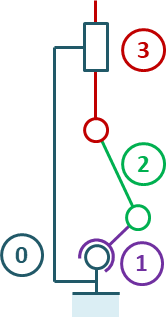
\includegraphics[width=3cm]{cas_08}
\end{center}
	\begin{reponses}	
	\bonne 1
	\mauvaise 0
	\mauvaise 2
	\mauvaise 3
	\end{reponses}
\end{question}\\}


\element{hs}{
\begin{question}{hs 09}
Soit le schéma suivant. Donner le degré d'hyperstatisme du mécanisme.
\begin{center}
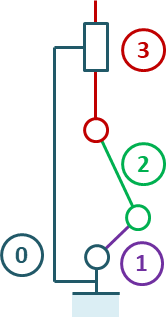
\includegraphics[width=3cm]{cas_09}
\end{center}
	\begin{reponses}	
	\bonne 3
	\mauvaise 0
	\mauvaise 2
	\mauvaise 1
	\end{reponses}
\end{question}\\}


\element{hs}{
\begin{question}{hs 10}
Soit le schéma suivant. Donner le degré d'hyperstatisme du mécanisme.
\begin{center}
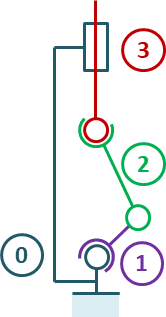
\includegraphics[width=3cm]{cas_10}
\end{center}
	\begin{reponses}	
	\bonne 0
	\mauvaise 1
	\mauvaise 2
	\mauvaise 3
	\end{reponses}
\end{question}\\}


\element{hs}{
\begin{question}{hs 11}
Soit le schéma suivant. Donner le degré d'hyperstatisme du mécanisme.
\begin{center}
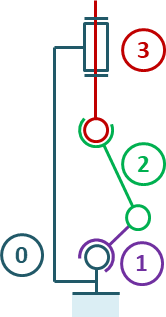
\includegraphics[width=3cm]{cas_11}
\end{center}
	\begin{reponses}	
	\bonne 0
	\mauvaise 1
	\mauvaise 2
	\mauvaise 3
	\end{reponses}
\end{question}\\}

\element{hs}{
\begin{question}{hs 12}
Soit le schéma suivant. Donner le degré d'hyperstatisme du mécanisme.
\begin{center}
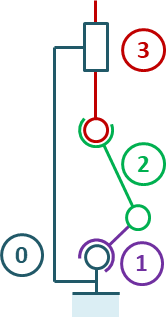
\includegraphics[width=3cm]{cas_12}
\end{center}
	\begin{reponses}	
	\bonne 0
	\mauvaise 1
	\mauvaise 2
	\mauvaise 3
	\end{reponses}
\end{question}\\}









\exemplaire{1}{
% Entetes sujet
\noindent{\bf QCM -- Hyperstatisme}

\vspace*{.5cm}
% Questions
\begin{multicols}{2}
\restituegroupe[4]{mob}
\restituegroupe[4]{hs}
\end{multicols}

\AMCcleardoublepage


\AMCdebutFormulaire
% ENtetes
{\large\bf Feuille de réponses :}
%
\vspace{.5cm}

\begin{minipage}[c]{.45\linewidth}
{\large\bf Noircir votre numéro personnel.}

\vspace{.5cm}

\AMCcodeGridInt[h]{etu}{2}
\end{minipage}
\hfill
\begin{minipage}[c]{.45\linewidth}
\champnom{\fbox{
\begin{minipage}{.9\linewidth}
Nom et prénom :

\vspace*{.5cm}\dotfill

\vspace*{.5cm}\dotfill

\vspace*{1mm}
\end{minipage}
}}
\end{minipage}

%%%%%%%

\vspace*{.5cm}
Pour répondre aux questions \textbf{noircir consciencieusement} la réponse sélectionnée. 
\vspace*{.5cm}

\formulaire
\AMCcleardoublepage
% 
}

\end{document}
